%-----------------------------------------------------------------------------%
\chapter{ANALISIS DAN PERANCANGAN SISTEM}
%-----------------------------------------------------------------------------%
\vspace{4.5pt}

\section{Analisis Masalah}
....

\begin{center}
	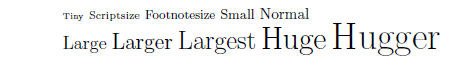
\includegraphics[width=8cm]{img/2.PNG}
	\captionof{figure}{...}
	\label{fig:asd}
\end{center}

\section{Kerangka Pemikiran}
\begin{center}
	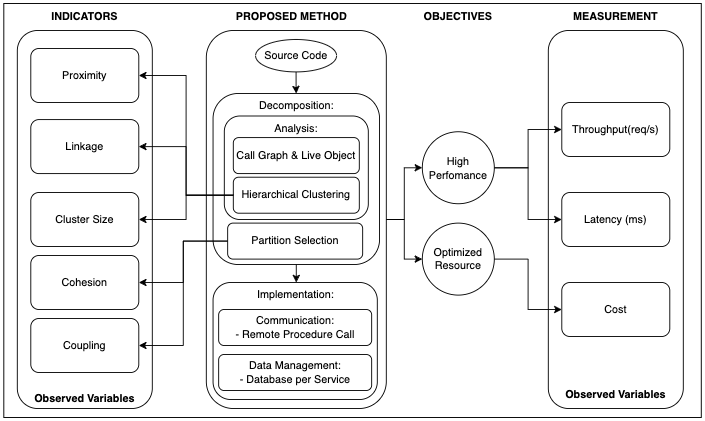
\includegraphics[width=14cm]{img/KerangkaPemikiran.png}
	\captionof{figure}{Kerangka Pemikiran}
	\label{fig:asd}
\end{center}

Penelitian akan dimulai dengan menggunakan kode sumber aplikasi yang dibuat dengan monolit. Kode sumber ini dilakukan proses dekomposisi yaitu dengan analisis seperti mencari objek beserta atributnya, untuk mencari keterhubungan lebih lanjut tentang objek maka dilakukan pencarian pada fungsi-fungsi sehingga terbentuklah grafik yang menunjukan bagaimana keterhubungan objek di aplikasi. \\

Dari grafik yang sudah dibuat akan dilakukan pengelompokan dengan pendekatan Hierarchical Clustering. Dimana perlu ditentukan jumlah cluster minimum yang harus ditemukan dan pemilihan algoritma Linkage. Metode linkage yaitu menentukan jarak atau kemiripan antara semua objek. Untuk menentukan jarak ini bisa dengan rata-rata, maximum, minimum dan mengecilkan variance. \\

Pengelompokan dari Hierarchical Clustering akan dipilih dengan mencari nilai cohesion terendah dan  nilai coupling tertinggi. Dimana Internal Coupling mengevaluasi tingkat ketergantungan langsung dan tidak langsung antar objek. Semakin banyak dua objek menggunakan metode masing-masing semakin mereka menjadi satu kesatuan. Sedangkan Internal Cohesion akan mengevaluasi kekuatan interaksi antar objek. Biasanya, dua objek atau lebih menjadi interaktif jika metodenya bekerja pada atribut yang sama.\\

Ketika analisis dekomposisi sudah selesai dilakukan maka akan dilakukan implementasi berdasarkan pengelompokannya masing-masing yang akan menjadi service. Untuk metode komunikasinya antara service yaitu dengan Remote Procedure Call(RPC) dan untuk mengelola data, setiap service memiliki databasenya masing-masing dan untuk menjaga konsistensi data antar service maka digunakan pendekatan SAGA dengan cara choreography.\\

Untuk mengetahui bagaimana performa dari microservice dibandingkan dengan monolit yaitu dengan test beban. Pengukuran performa dilihat dari throughput, jumlah response, dan latency. 


\section{Urutan Proses Global}
\begin{center}
	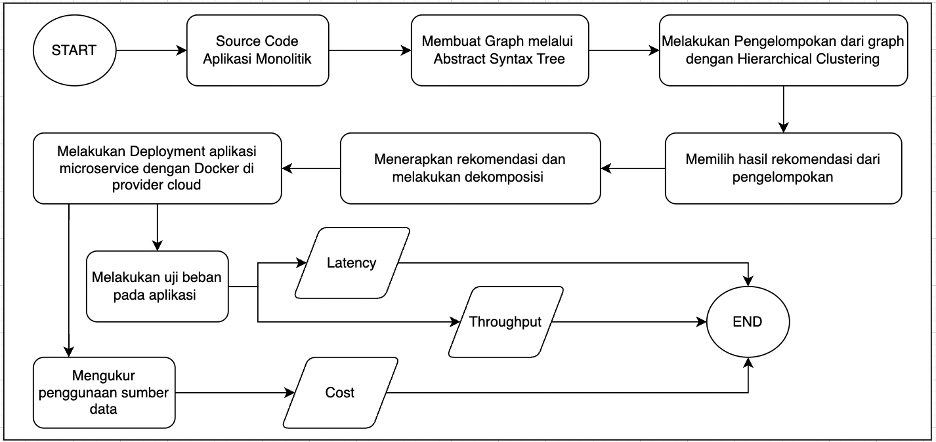
\includegraphics[width=14cm]{img/FlowchartProsesGlobal.png}
	\captionof{figure}{Diagram Flowchart Proses Global }
	\label{fig:asd}
\end{center}
.....


\section{Analisis Manual}
....

\begin{small}
    \begin{longtable}[c]{|l|l|l|l|}
		\caption{Tabel complex}\\
		\hline
        \multirow{10}{*}{numeric literals} & \multirow{5}{*}{integers} & in decimal & \verb|8743| \\ \cline{3-4}
        & & \multirow{2}{*}{in octal} & \verb|0o7464| \\ \cline{4-4}
        & & & \verb|0O103| \\ \cline{3-4}
        & & \multirow{2}{*}{in hexadecimal} & \verb|0x5A0FF| \\ \cline{4-4}
        & & & \verb|0xE0F2| \\ \cline{2-4}
        & \multirow{5}{*}{fractionals} & \multirow{5}{*}{in decimal} & \verb|140.58| \\ \cline{4-4}
        & & & \verb|8.04e7| \\ \cline{4-4}
        & & & \verb|0.347E+12| \\ \cline{4-4}
        & & & \verb|5.47E-12| \\ \cline{4-4}
        & & & \verb|47e22| \\ \cline{1-4}
        \multicolumn{3}{|l|}{\multirow{3}{*}{char literals}} & \verb|'H'| \\ \cline{4-4}
        \multicolumn{3}{|l|}{} & \verb|'\n'| \\ \cline{4-4}          %% here
        \multicolumn{3}{|l|}{} & \verb|'\x65'| \\ \cline{1-4}        %% here
        \multicolumn{3}{|l|}{\multirow{2}{*}{string literals}} & \verb|"bom dia"| \\ \cline{4-4}
        \multicolumn{3}{|l|}{} & \verb|"ouro preto\nmg"| \\ \cline{1-4}          %% here
	\end{longtable}
\end{small}
